\chapter{Netzteil}
\label{ch:Netzteil}

\section{Allgemeines}
Um eine fehlerfreie Funktion aller weiteren Module zu gewährleisten, ist es wichtig, dass eine geeignete Spannungsversorgung bereitgestellt wird. 
Insbesondere für die Opamp-Schaltungen ist es wichtig, dass eine störfreie symmetrische Spannung bereitgestellt wird. 
Im Bereich der modularen Synthesizer wird hier typischerweise eine Spannung von +/- 12 V benötigt. Diese Spannungspegel werden durch eine geignete Beschaltung von Dioden und Kondensatoren generiert, welche in Abschnitt \ref{sec:Netzteil_Schaltplan} bzw. \ref{sec:Netzteil_Umsetzung} bildlich erläutert werden. Hierbei wird die für modulare Synthesizer typischerweise eingesetzte Wannenstecker-Belegung verwendet. Diese wird entsprechend in allen weiteren Modulen eingesetzt!

\newpage

\FloatBarrier
\section{Schaltplan}
\label{sec:Netzteil_Schaltplan}

\begin{figure}[h]
\centering
\setlength{\fboxsep}{1pt} %Abstand der Linien zur Abbildung
\setlength{\fboxrule}{1pt} %Dicke der Linie
\fbox{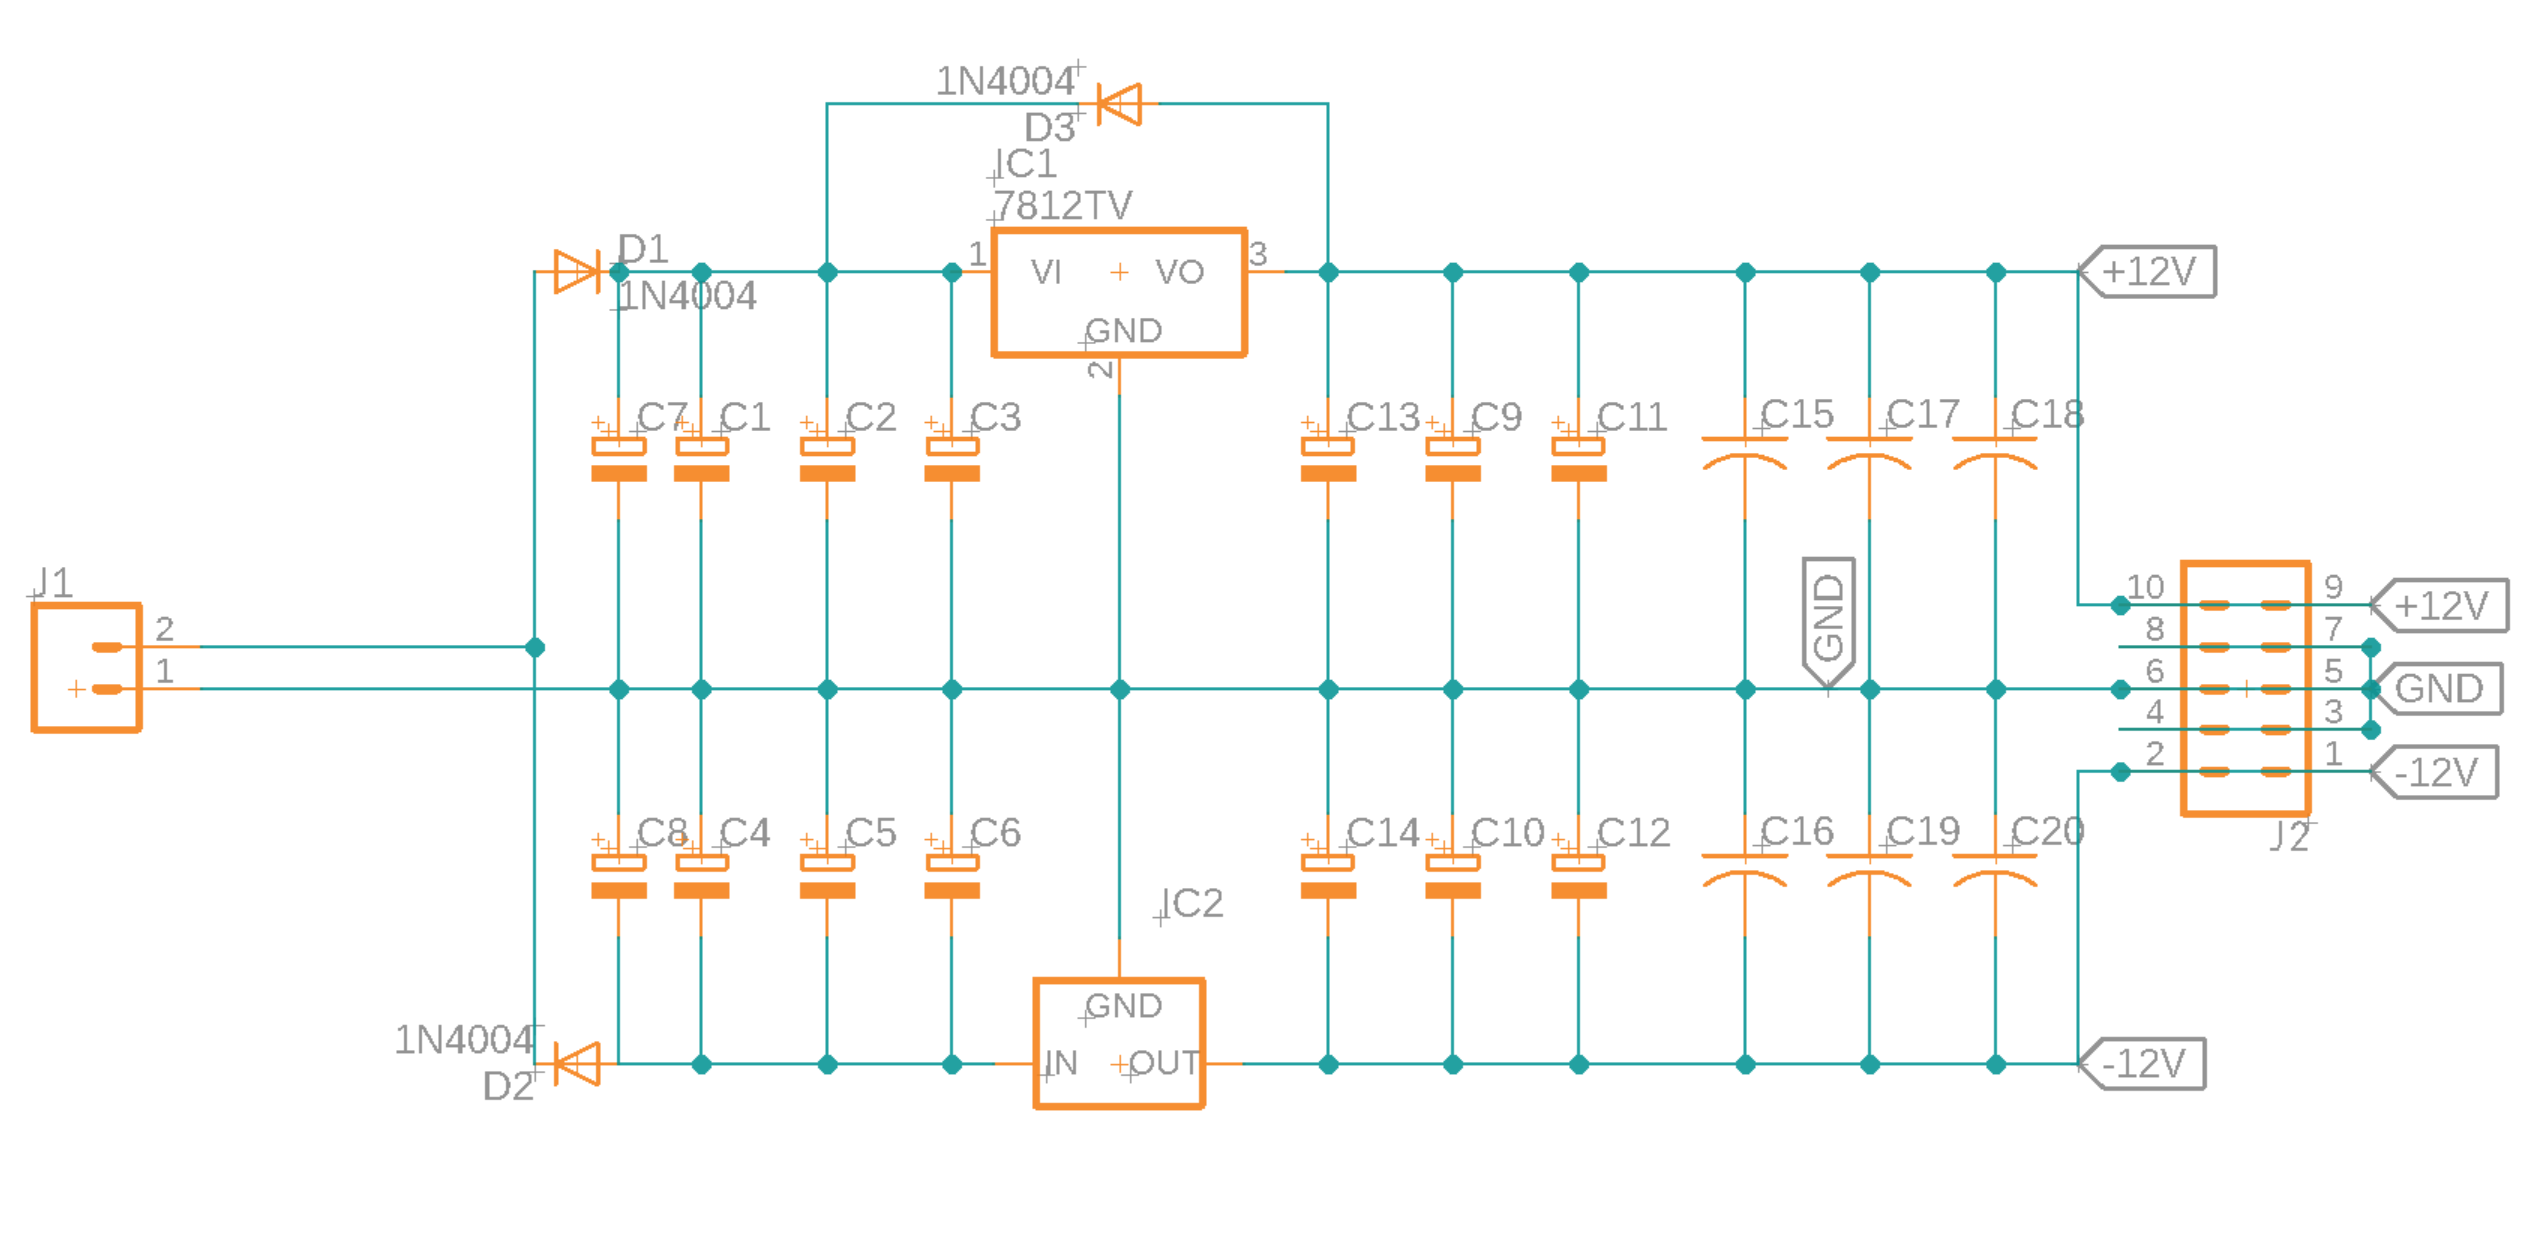
\includegraphics[width=1\textwidth]{figures/Schaltplan_Netzteil.png}}
\caption{Fusion360 Schaltplan des Netzteils}
\label{fig:Netzteil_Schaltplan}
\end{figure}
\FloatBarrier

\FloatBarrier
\section{Umsetzung}
\label{sec:Netzteil_Umsetzung}

\begin{figure}[h]
\setlength{\fboxsep}{1pt} %Abstand der Linien zur Abbildung
\setlength{\fboxrule}{1pt} %Dicke der Linie
\fbox{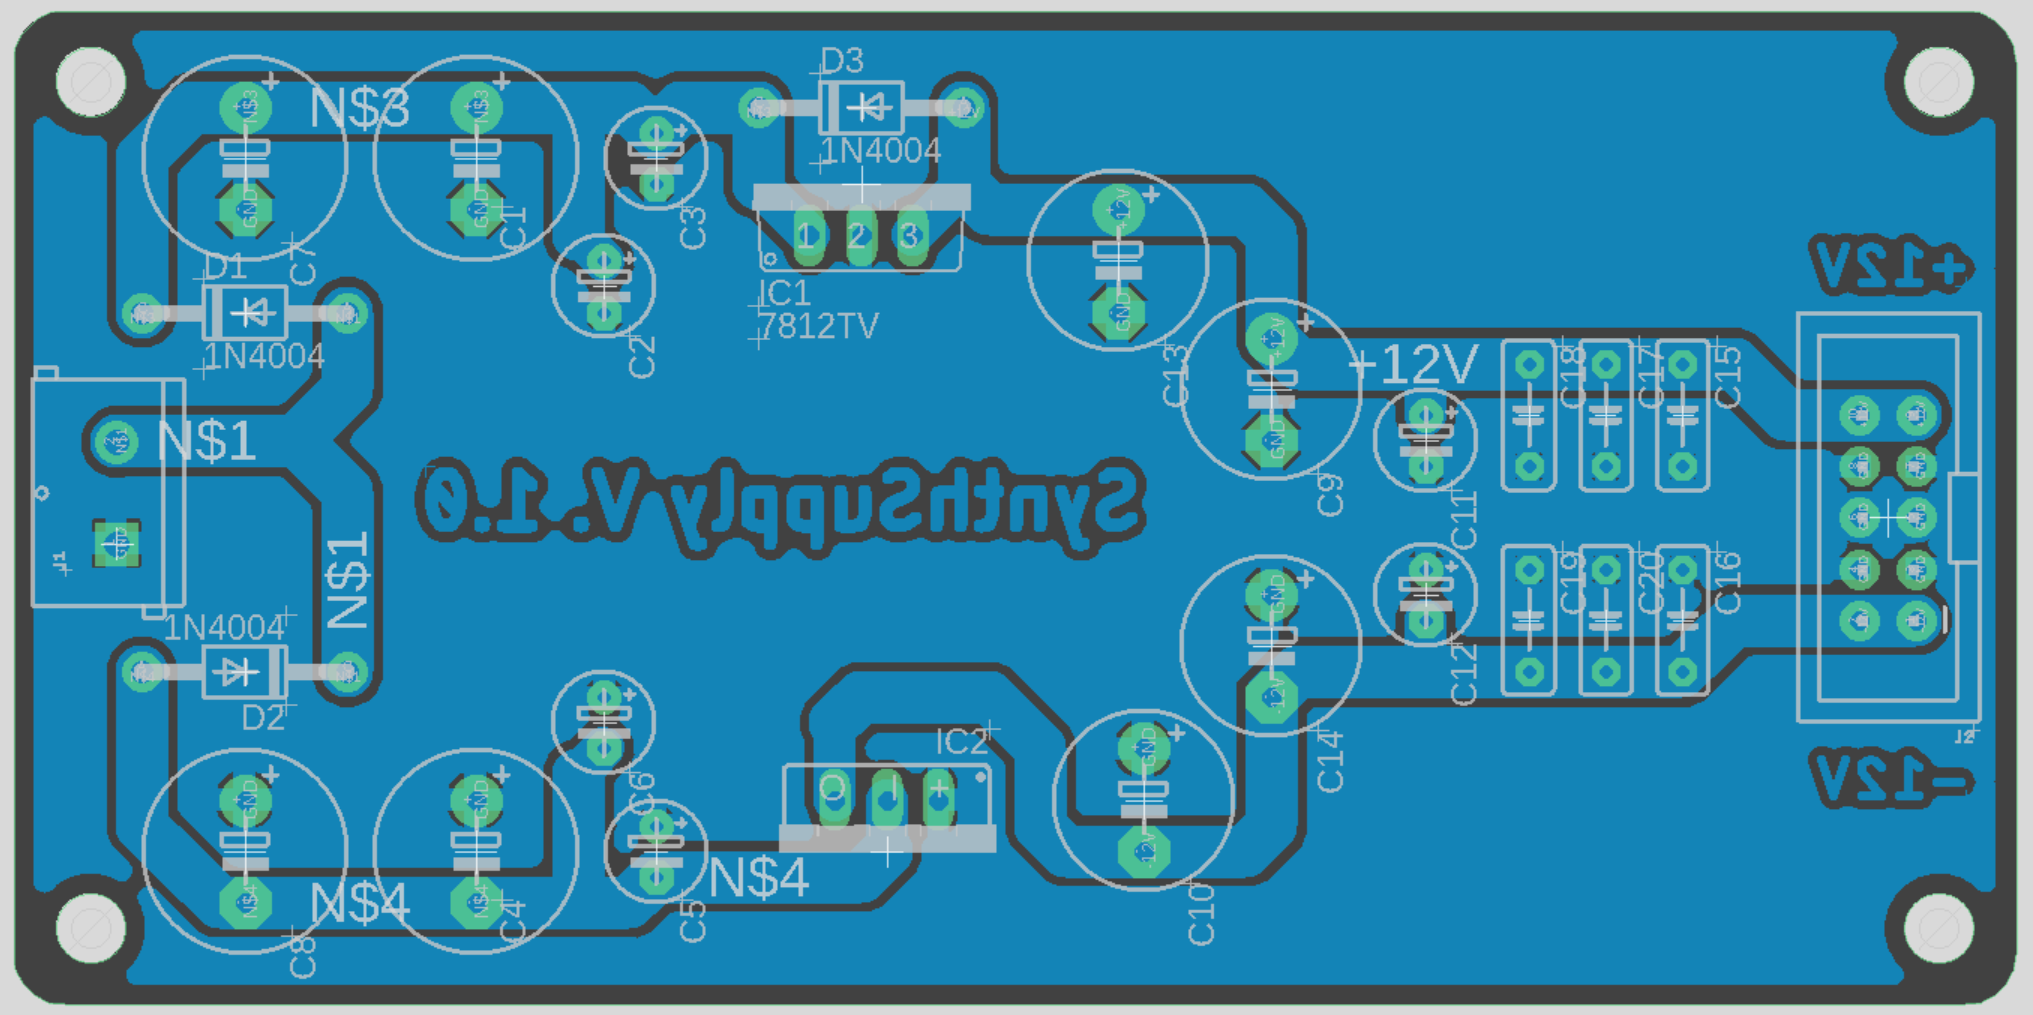
\includegraphics[width=1\textwidth]{figures/Layout_Netzteil.png}}
\caption{Fusion360 Schaltplan des Netzteils}
\label{fig:Netzteil_Layout}
\end{figure}
\FloatBarrier